\documentclass{article}

\usepackage{graphicx}
\usepackage{tikz}
\usepackage{tikzsymbols}
\usetikzlibrary{calc,patterns,shapes.geometric}
\pagestyle{empty}
\usepackage[margin=0pt]{geometry}
\geometry{papersize={14in,12in}}

\def\centerarc[#1](#2)(#3:#4:#5){\draw[#1] ($(#2)+({#5*cos(#3)},{#5*sin(#3)})$) arc (#3:#4:#5);}

\begin{document}
	\begin{figure}
		\centering
		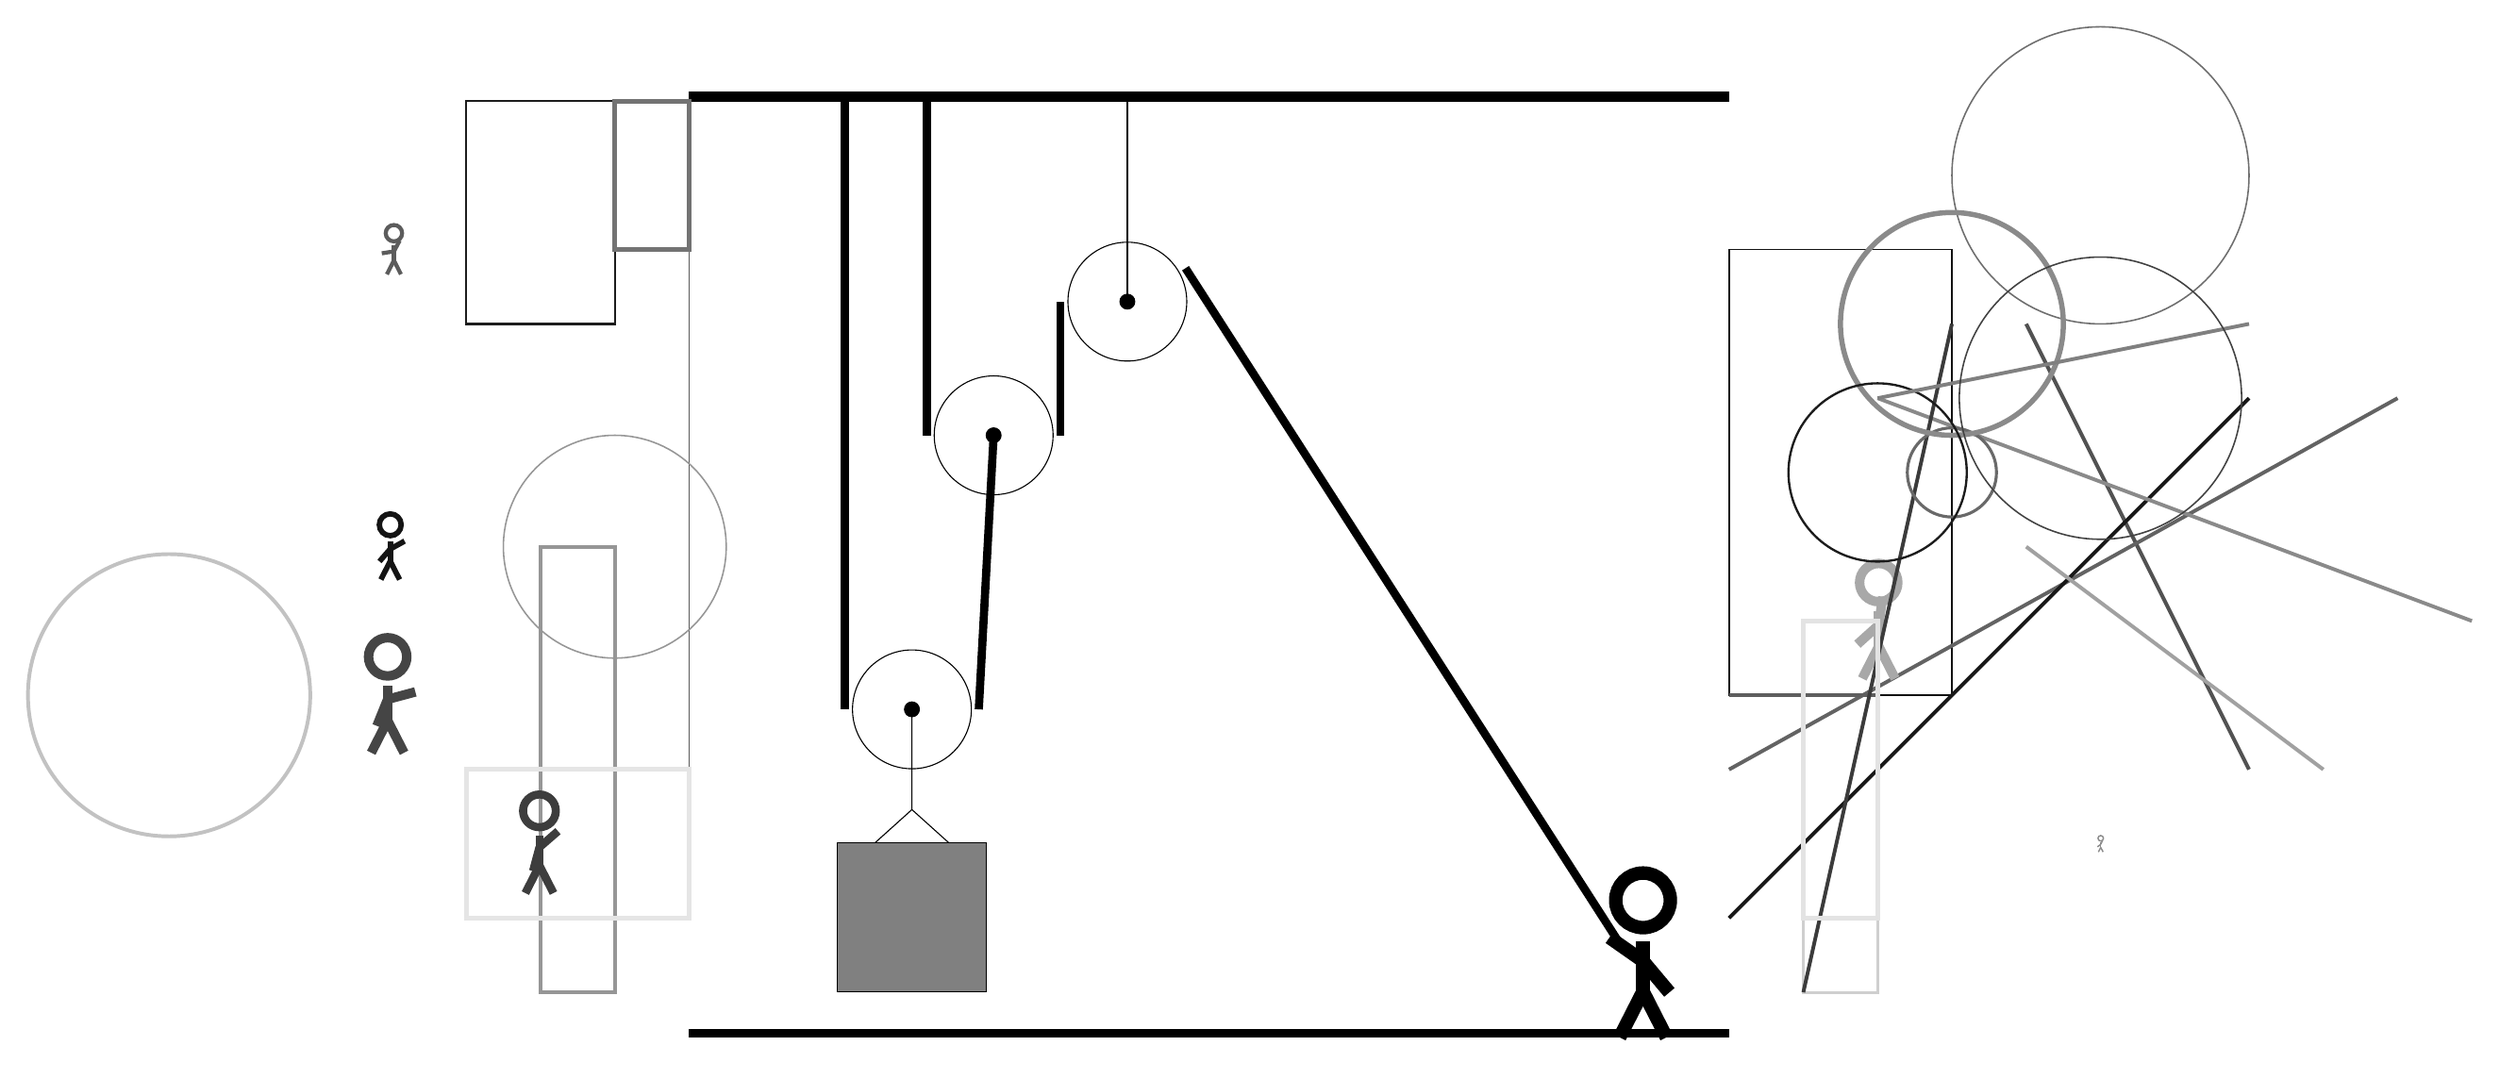
\begin{tikzpicture}
			%%%%% START %%%%%
			
			\draw[fill=black] (-2, 9) rectangle (12, 9.125);
			
			\draw (1, 0.81) circle (0.8);
			\draw[fill=black] (1, 0.81) circle (0.1);
			
			\draw (2.1, 4.5) circle (0.8);
			\draw[fill=black] (2.1, 4.5) circle (0.1);
			
			\draw[line width=0.2mm, color=black!93] (12, 7) rectangle (15, 1);
			
			\draw[line width=0.4mm, color=black!19] (14, 1) rectangle (13, -3);
			\draw[line width=0.2mm, color=black!65] (-2, 8) rectangle (-2, 0);
			\draw[line width=0.5mm, color=black!68](16, 6) -- (19, 0);
			
			\node[line width=0.7mm, color=black!64] at (-6, 7) {\Strichmaxerl[3][9][62]};
			\draw[line width=0.5mm, color=black!41] (-4, 3) rectangle (-3, -3);
			\draw[line width=0.3mm, color=black!89] (-3, 6) rectangle (-5, 9);
			\draw[line width=0.5mm, color=black!61](12, 0) -- (21, 5);
			\draw[line width=0.5mm, color=black!63] (12, 1) rectangle (14, 1);
			\draw [line width=0.2mm, color=black!57](17, 8) circle (2.0);
			
			\draw[line width=0.5mm, color=black!90](12, -2) -- (19, 5);
			\draw[line width=0.5mm, color=black!46](14, 5) -- (22, 2);
			\draw[line width=0.6mm, color=black!55] (-3, 9) rectangle (-2, 7);
			
			\node[line width=0.2mm, color=black!73] at (-6, 1) {\Strichmaxerl[7][68][15]};
			\node[line width=0.2mm, color=black!34] at (14, 2) {\Strichmaxerl[7][42][82]};
			\draw [line width=0.2mm, color=black!41](-3, 3) circle (1.5);
			\draw [line width=0.5mm, color=black!24](-9, 1) circle (1.9);
			\draw[line width=0.5mm, color=black!77](13, -3) -- (15, 6);
			\draw [line width=0.4mm, color=black!59](15, 4) circle (0.6);
			\draw[line width=0.6mm, color=black!10] (-2, 0) rectangle (-5, -2);
			\draw[line width=0.5mm, color=black!37](16, 3) -- (20, 0);
			
			\node[line width=0.5mm, color=black!76] at (-4, -1) {\Strichmaxerl[6][75][41]};
			\draw [line width=0.7mm, color=black!46](15, 6) circle (1.5);
			\draw [line width=0.3mm, color=black!89](14, 4) circle (1.2);
			\node[line width=0.3mm, color=black!45] at (17, -1) {\Strichmaxerl[1][37][65]};
			\draw[line width=0.5mm, color=black!50](14, 5) -- (19, 6);
			\draw[line width=0.7mm, color=black!11] (13, -2) rectangle (14, 2);
			\node[line width=0.2mm, color=black!92] at (-6, 3) {\Strichmaxerl[4][49][29]};
			\draw [line width=0.2mm, color=black!74](17, 5) circle (1.9);
			
			\draw (3.9, 6.3) circle (0.8);
			\draw[fill=black] (3.9, 6.3) circle (0.1);
			\draw[thick] (3.9, 6.3) -- (3.9, 9);
			
			\draw (1, 0.81) -- (1, -0.54) -- (0.5, -0.99) -- (1.5, -0.99) -- (1, -0.54);
			\draw[fill=black!50] (0, -0.99) rectangle (2, -2.99);
			
			\draw[line width=1.1mm] (0.1, 9) -- (0.1, 0.81);
			\centerarc[line width=1.1mm](1, 0.81)(180:360:0.9);
			\draw[line width=1.1mm](1.9, 0.81) -- (2.1, 4.5);
			\draw[line width=1.1mm] (1.2, 9) -- (1.2, 4.5);
			\centerarc[line width=1.1mm](2.1, 4.5)(180:360:0.9);
			\draw[line width=1.1mm](3.0, 4.5) -- (3.0, 6.3);
			\centerarc[line width=1.1mm](3.9, 6.3)(30:180:0.9);
			\draw[line width=1.1mm] (4.683, 6.75) -- (10.5, -2.3);
			
			\node at (10.8, -2.5) {\Strichmaxerl[10][-35][-50]};
			
			\draw[fill=black] (-2, -3.5) rectangle (12, -3.6);
			
			%%%%% END %%%%%
		\end{tikzpicture}
	\end{figure}	
\end{document}